%\documentclass[aps,prl,reprint,groupedaddress,preprint]{revtex4-2}
\documentclass{article}
\usepackage[a4paper,margin=2cm]{geometry}
\usepackage{amsmath,amssymb}
\usepackage{tikz}
\usepackage{braket}
\newcommand{\RR}{\mathbb{R}}
\newcommand{\CC}{\mathbb{C}}
\newcommand{\pdiff}[2]{\frac{\partial #1}{\partial #2}}


\begin{document}

% Title, authors, abstract, etc.

\title{Finite Difference Method in Polar Coordinates}
\author{Simen Kvaal}
%\affiliation{Hylleraas Centre for Quantum Molecular Sciences, Department of Chemistry, University of Oslo, P.O. Box 1033 Blindern, N-0315 Oslo, Norway}

\begin{abstract}
This note describes the finite difference method in polar coordinates.
\end{abstract}

\maketitle

% Main body of the document

\section{Weak formulation of the Schr\"odinger equation}

We consider the solution of the Schr\"odinger equation for a particle in two dimensions,
\begin{equation}
    H\psi(\mathbf{r}) = -\frac{1}{2} \nabla^2 \psi + V(\mathbf{r}) \psi(\mathbf{r}) = E \psi(\mathbf{r}),
\end{equation}
where $\mathbf{r} \in D = \{ \mathbf{r}| < r_\text{max} \}$, the disk with radius $r_\text{max}$, and where $V(\mathbf{r})$ is assumed to be smooth. It is a well-known fact that any eigenfunction $H$ must possess is then smooth, and that $H$ is self-adjoint over $L^2(D)$ with domain $H^2(D)$. Furthermore, the boundedness of $D$ implies that $H$ has a purely discrete spectrum and a complete set of eigenfunctions.

The \emph{weak formulation} passes to a sesquilinear form $h : H^1(D)\times H^1(D) \to \CC$ defined using integration by parts on smooth functions,
\begin{equation}
    h(\phi,\psi) = \frac{1}{2} \int_D \nabla \phi(\mathbf{r}) \cdot \nabla \psi(\mathbf{r}) \; d\mathbf{r} + \int_D V(\mathbf{r}) \phi(\mathbf{r}) \psi(\mathbf{r}) \; d\mathbf{r}.
\end{equation}
The eigenvalues of $H$ are now the critical points of the Rayleigh quotient defined by
\begin{equation}
    \mathcal{E}(\psi) = \frac{h(\psi,\psi)}{\braket{\psi,\psi}}.
\end{equation}
If we select a family $V_h \subset H^1(D)$ of finite-dimensional subspaces, such that $V_h \to H^1(D)$ as $h\to 0$, then the variational Galerkin approximation is defined by locating the critical points of $\mathcal{E}$ over $V_h$. For any choice $\{\phi_k\}\subset V_h$ of basis functions, this is equivalent to the matrix eigenvalue problem
\begin{equation}
    \mathsf{H} \mathsf{c} = E_h \mathsf{S} \mathsf{c},
\end{equation}
where $\mathsf{H} = \mathsf{H}^H$ has matrix elements $\mathsf{H}_{k,l} = h(\phi_k,\phi_l)$, $\mathsf{S} = \mathsf{S}^H$ has matrix elements $\mathsf{S}_{k,l} = \braket{\phi_k,\phi_l}$, and $\psi_h = \sum_k \mathsf{c}_k \phi_h$ is the approximate eigenfunction.

The eigenvalues of $\mathsf{H}_h$ converge to the eigenvalues of $H$ as $h\to 0$, and the eigenfunctions converge to the eigenfunctions of $H$ in the $H^1(D)$ norm.

\section{Polar coordinates}

We introduce polar coordinates $(x,y) = (r\cos\theta,r\sin\theta)$ and the volume element becomes
\begin{equation}
    d\mathbf{r} = r dr d\theta.
\end{equation}
The gradient operator in polar coordinates is given by:
\begin{equation}
    \nabla = \frac{\partial}{\partial r} \hat{\mathbf{r}} + \frac{1}{r} \frac{\partial}{\partial \theta} \hat{\boldsymbol{\theta}}.
\end{equation}
Here, $\hat{\mathbf{r}}$ is the unit vector in the radial direction, and $\hat{\boldsymbol{\theta}}$ is the unit vector in the angular direction. These vectors are orthogonal. As a result, the form $h$ becomes
\begin{equation}
    h(\phi,\psi) = \frac{1}{2} \int_D \pdiff{\phi^*}{r} \pdiff{\psi}{r} + \frac{1}{r^2} \pdiff{\phi^*}{\theta} \pdiff{\psi}{\theta} + V \phi^* \psi  \; r \, dr \, d\theta. \label{eq:form-polar}
\end{equation}
We note that the Laplace--Beltrami operator in polar coordinates is
\begin{equation}
  \nabla^2 =
\frac{1}{r} \frac{\partial}{\partial r} \left( r \frac{\partial}{\partial r} \right) + \frac{1}{r^2} \frac{\partial^2}{\partial\theta^2},
\end{equation}
and that Eq.~\eqref{eq:form-polar} can be obtained using this formula and integration by parts. In particular, the Schrödinger equation on strong form in polar coordinates is
\begin{equation}
    -\frac{1}{2} \left( \frac{1}{r} \frac{\partial}{\partial r} \left( r \frac{\partial}{\partial r} \right) - \frac{1}{r^2} \frac{\partial^2}{\partial\theta^2} \right) \psi + V \psi = E \psi.
\end{equation}

The next step is to introduce a Fourier expansion in the angular direction,
\begin{equation}
    \psi(r,\theta) = \sum_{m=-\infty}^\infty e^{im\theta} \psi_m(r).
\end{equation}
Since $\psi$ is assumed smooth, the Fourier coefficients $\psi_m(r)$ are smooth functions of $r$, and at the coordinate singularity $r=0$, we have the boundary condition $\psi_0'(0) = 0$ and $\psi_m(0) = 0$ for $m\neq 0$. The radial functions $\psi_m(r)$ are
elements of $L^2([0, r_\text{max}], r dr)$, on which the inner product is
\begin{equation}
    \braket{u,v}_r = \int_0^{r_\text{max}} u(r)^* v(r)\;  r dr.
\end{equation}
Similarly, the potential $V(r,\theta)$ is expanded as
\begin{equation}
    V(r,\theta) = \sum_{m=-\infty}^\infty e^{im\theta} V_m(r).
\end{equation}
The boundary conditions at $r=0$ are the same for $V_m$ as for $\psi_m$.


Inserting the Fourier expansions into the Schr\"odinger equation, we obtain
\begin{equation}
 H\psi = \sum_m e^{im\theta}\left[  
        -\frac{1}{2} \left( \frac{1}{r} \frac{\partial}{\partial r} \left( r \frac{\partial}{\partial r} \right) + \frac{m^2}{2r^2} \right)
        \right]\psi_m(t) + \sum_{m,m'} e^{i(m+m')\theta} V_{m'}(r) \psi_{m}(r) .
\end{equation}
Fourier decomposing $H\psi = \sum_m e^{i m\theta} (H\psi)_m$ and integrating against $e^{-im\theta}$ gives
\begin{equation}
    (H\psi)_m = T_m \psi_m(t) + \sum_{m'} V_{m-m'}(r) \psi_{m'}(r) .
\end{equation}
where
\begin{equation}
 T_m = -\frac{1}{2} \frac{1}{r} \frac{\partial}{\partial r} \left( r \frac{\partial}{\partial r} \right) + \frac{m^2}{2r^2} .
\end{equation}
The sesquilinear form $h$ becomes
\begin{equation}
    \begin{split}
    h(\phi,\psi) &= \frac{1}{2} \sum_m \braket{\partial_r \phi_m, \partial_r \psi_m}_r + \frac{1}{2} \sum_m m^2 \braket{\phi_m,r^{-2}\psi_m}_r + \sum_{m,m'} \braket{\phi_m, V_{m-m'} \psi_{m'}}_r \\
    &= t_0(\phi,\psi) + v^{\text{centrifugal}}(\phi,\psi) + v(\phi,\psi) \\
    &= t_m(\phi,\psi) + v(\phi,\psi) \label{eq:form-polar}
    \end{split}
\end{equation}

It is useful for later reference to do the integration by parts transition from $T_0$ to the form $t_0$ defined by the first term of Eq.~\eqref{eq:form-polar}. This gives:
\begin{equation}
-2\braket{u,T_0v}_r =  \braket{u, (r^{-1}\partial_r r\partial r) v}_r = \int u^*(r) \partial_r (r \partial_r v) \; dr = 
    \left[ u^*(r) \partial_r v(r) r  \right]_0^\infty - \int \partial_r u^*(r) \partial_r v(r) r \; dr.
\end{equation}
The boundary terms vanish if $u$ and $v$ are sufficiently regular. We therefore obtain the
sesquilinear form
\begin{equation}
    t_0(u,v) = \frac{1}{2}\braket{ \partial_r u, \partial_r v}_r.
\end{equation}

The form $h$ is bounded and coercive on the domain $H^1(\RR^2)$ of $h$,
\begin{equation}
    |h(\phi,\psi)| \leq C \|\phi\|_{H^1(D)} \|\psi\|_{H^1(D)}, \qquad h(\phi,\phi) \geq c \|\phi\|_{H^1(D)}^2.
\end{equation}

\section{Finite element method}

We introduce linear finite elements in the radial coordinate: we  divide $[0, r_\text{max}]$ into $n+1$ uniform intervals of length $h = r_\text{max}/(n+1)$. The nodes of the grid are thus $r_k = kh$ for $k=0,1,\ldots,n+1$, in total $n+2$ points. We will enforce (discrete) boundary conditions at $r=0$ and $r=r_\text{max}$, so that the total number of degrees of freedom for a radial wavefunction is $n$.

We introduce the space of piecewise linear and continuous functions $V_h$ over $[0, r_\text{max}]$. These functions are weakly differentiable, with derivatives that are constant over the intervals. Thus, $V_h \subset H^1([0,r_\text{max}];r dr)$. The space of derivatives is denoted $W_h \subset L^2([0,r_\text{max}]; r dr)$.

A basis for $V_h$ is given by the hat functions $u_k$, for $k=0,1,\ldots,n+1$, defined by
\begin{equation}
    u_k(r) = \begin{cases}
        \frac{r-r_{k-1}}{h} & r_{k-1} \leq r \leq r_k, \\
        \frac{r_{k+1}-r}{h} & r_k \leq r \leq r_{k+1}, \\
        0 & \text{otherwise}.
    \end{cases}
\end{equation}
See~\ref{fig:fem-basis} for an illustration.
We note that $k=0$ and $k=n+1$ are special, in that the functions $u_0$ and $u_{n+1}$ are nonzero only on the interval $[0,h]$ and $[r_\text{max}-h,r_\text{max}]$, respectively, and does not have the hat shape.


The functions satisfy $u_k(r_j) = \delta_{k,j}$, and we note that the exact derivative of $u_k$ is given by the forward difference formula: For $x \in [x_k, x_{k+1}]$, we have $u'_k(x) = h^{-1} (u_{k+1}(x) - u_k(x))$.

The finite element method is now completed by evaluating the form $h$ on the basis functions $u_k$ and $u_l$, yielding $\mathsf{H}_{k,l}$, as well as the overlap matrix $\mathsf{S}_{k,l} = \braket{u_k,u_l}_r$. 

The kinetic energy terms and overlap integrals are obtained by analytic integration, since the basis functions are piecewise linear. The potential energy terms are obtained by numerical integration. 

We will enforce homogenous Dirichlet BCs at the right endpoint homogenous Neumann conditions at the left endpoint for $m=0$, and homogenous Dirichlet conditions otherwise. In both cases, the basis function $u_0$ is eliminated, resulting in a modified basis of $n$ functions $\tilde{u}_k$, where we choose to start numbering at $k=1$. The elimination produces a matrix $\mathsf{G} \in \RR^{n+2,n}$ such that
\begin{equation}
    \tilde{u}_k = \sum_{k'=0}^{n+1} u_{k'} \mathsf{G}_{k',k} .
\end{equation}
Let now $a$ be sesquilinear form on $V_h$ (i.e., it does not coupled different $m$ values). Evaluating the form on the modified basis functions $\tilde{u}_k$ is equivalent to evaluating the form on the original basis functions $u_k$ and multiplying the result by $\mathsf{G}^T$ from the left and $\mathsf{G}$ from the right. That is,
\begin{equation}
    \mathsf{A}_{k,l} := a(\tilde{u}_k, \tilde{u}_l) = \sum_{k',l'} \mathsf{G}_{k',k} \mathsf{G}_{l',l} a(u_{k'}, u_{l'}) = \sum_{k',l'} \mathsf{G}_{k',k} \mathsf{G}_{l',l} \mathsf{A}_{k',l'} = (\mathsf{G}^T \mathsf{A}_0 \mathsf{G})_{k,l},
\end{equation}
where $\mathsf{A}_0$ is the form matrix on the FEM basis witout boundary conditions. 

The matrix $G$ is easy to find. For $m\neq 0$, the homogenous Dirichlet conditions imply that the coefficients of $u_0$ and $u_{n+1}$ in the wavefunction must be zero. This gives $\mathsf{G}_{0,:} = \mathsf{G}_{n+1,:} = 0$, and $\mathsf{G}_{1:n+1, 1:n+1} = I_n$. For $m=0$, the Neumann condition at $r=0$ means that we must require $\psi'(0) = 0$. This implies that the coefficients of $u_0$ and $u_1$ must be equal. Thus, $\mathsf{G}$ is as before, except for the matrix element $\mathsf{G}_{0,1} = 1$.


We now outline the assembly of the full coupled system. For each $m$ we have an independent basis set $\tilde{u}^m_k$ of $n$ functions, and correspondingly
\begin{equation}
    \psi = \sum_m \sum_k c_k^m \tilde{u}^m_k.
\end{equation}
Similarly, we have matrices $\mathsf{G}^m$ for each $m$. The matrix of the kinetic energy is then block diagonal, with the potential matrix coupling different $m$. We obtain
\begin{equation}
    (\mathsf{H} \mathsf{c})^m = \mathsf{T}^m \mathsf{c}^m + \sum_{m'} \mathsf{V}^{m,m'} \mathsf{c}^{m'}.
\end{equation}
Here,
\begin{equation}
    \mathsf{T}^m = \mathsf{G}^{m,T} \mathsf{T}_{m,0} \mathsf{G}^m
\end{equation} 
where $\mathsf{T}_{m,0}$ is the kinetic energy matrix for the given $m$ without boundary conditions. Similarly,
\begin{equation}
    \mathsf{V}^{m,m'} = \mathsf{G}^{m,T} \mathsf{V}_{m-m',0} \mathsf{G}^{m'}
\end{equation} 
where we note the presence of different angular momentum numbers. Finally, the overlap matrix is block diagonal, with blocks
\begin{equation}
    \mathsf{S}^{m} = \mathsf{G}^{m,T} \mathsf{S}_0 \mathsf{G}^m.
\end{equation}






In the next section we prove that the kinetic energy matrix is identical to the finite difference kinetic energy matrix obtained with a particular scheme, and that ``lumping'' the overlap matrix yields the finite difference overlap matrix, which is diagonal. (Lumping is the process of replacing the full overlap matrix with a diagonal matrix where the columns are summed and placed on the diagonal.) Finally, the potential matrix is identical to the finite difference potential matrix when the trapezoidal rule is used for numerical integration.

\begin{figure}[htbp]
    \centering
    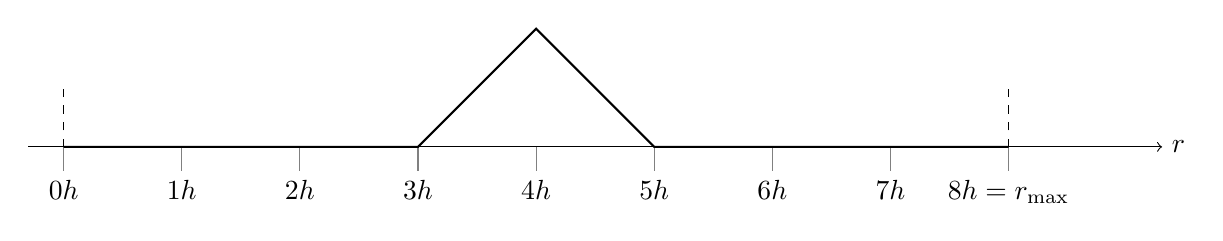
\begin{tikzpicture}[scale=1.5]

        \newcommand{\N}{8}
        \foreach \x in {0,...,\N} {
            \draw[gray] (\x,0) -- (\x,-0.2);
            \ifnum\x=\N
                \node[below] at (\x,-0.2) {$\N h = r_\text{max}$};
            \else
                \node[below] at (\x,-0.2) {$\x h$};
            \fi
        }
        \draw[dashed] (0,0) -- (0,0.5);
        \draw[dashed] (\N,0) -- (\N,0.5);

        % \draw[gray] (0,0) -- (0,0.2);
        % \node[above] at (0,0.2) {$0$};
        
        % \draw[gray] (1,0) -- (1,0.2);
        % \node[above] at (1,0.2) {$h$};
        
        % \draw[gray] (2,0) -- (2,0.2);
        % \node[above] at (2,0.2) {$2h$};
        
        % \draw[gray] (3,0) -- (3,0.2);
        % \node[above] at (3,0.2) {$3h$};
        
        \newcommand{\K}{4}
        \draw[thick] (0,0) -- (\K-1,0) -- (\K,1.0) -- (\K+1,0) -- (\N,0);
             

        % Axis arrow
        \draw[->] (-0.3,0) -- (\N+1.3,0) node[right] {$r$};

    \end{tikzpicture}
    \caption{Finite element method hat function. The value at the peak is $1$.}
    \label{fig:fem-basis}
\end{figure}






\section{Finite difference method}


The finite difference method differs from the finite element method in that it
does not start with a variational formulation. Instead, it starts with a grid and a collocation idea, i.e., that the unknown function is assumed to be exactly known at the grid. The derivative operators are replaced by difference formulas, and potential terms become diagonal operators using collocation.

In our 2d probolem, we need a dicretization of the radial Laplacian,
\begin{equation}
    L_0 = \frac{1}{r} \frac{\partial}{\partial r} \left( r \frac{\partial}{\partial r} \right).
\end{equation}
The basic recipe to obtain a finite difference approximation is to define a central difference $\delta_h$ of total width $h$ and replace verbatim in $L_r$, i.e.,
\begin{equation}
    \delta_h f(x) = \frac{f(x+h/2) - f(x-h/2)}{h}.
\end{equation}
Applicaton of $\delta_h$ \emph{once} gives a result living ``off-grid'' so to speak, but application twice gives a 3-point formula of grid evaluation only. In our case,
\begin{equation}
    \delta_h f(r) = h^{-1}[f(r+h/2) - f(r-h/2)]
\end{equation}
\begin{equation}
    r \delta_h f(r) = h^{-1} r [f(r+h/2) - f(r-h/2)]
\end{equation}
\begin{equation}
    L_{0,h} = r^{-1} \delta_h r \delta_h f(r) = h^{-2} r^{-1} \{ (r+h/2) [f(r+h) - f(r)] - (r-h/2) [f(r) - f(r-h)] \}.
\end{equation}
This defines the finite difference approximation of $L_0$. Its matrix is readily obtained.

It is now interesting to observe, that this finite difference approximation is \emph{identical} to the FEM approximation described above! Since the FEM basis functions are piecewise linear, their derivatives are exactly given by the finite difference formula,
\begin{equation}
    u_k'(r_k + h/2) = \delta_h u_k(r_k + h/2).
\end{equation}
Since the derivatives are piecewise constant, $t_0(u_k,u_l)$ is the integral of a piecewise \emph{linear} function due to the volume element $r dr$. This function is exactly integrated by the trapezoidal rule,
\begin{equation}
    \int_{x_k}^{x_{k+1}} f(x) \; dx = \frac{h}{2} [f(x_k) + f(x_{k+1})].
\end{equation}
When $f(x)$ is linear over the interval, the trapezoidal rule is exact.

Define $a_{kl}^j$ as the value of $u'_k(r) u'_j(r)$ inside the interval $[r_j,r_{j+1}]$, a constant. In particular, it is the value at $r_j+h/2$. Then,
\begin{equation}
    2t_0(u_k,u_{l}) = \int u_k'(r) u_l'(r) r \; dr = \sum_{j=0}^{n} a_{kl}^{j} \int_{r_j}^{r_{j+1}} r dr  = \sum_{j=0}^{n} a_{kl}^j (r_j + h/2) = \sum_{j=0}^{n} \delta_h u_k(r + h/2) \delta_h u_l(r + h/2) \cdot (r + h/2).
\end{equation}
For grid functions $f(x_j)$ and $g(x_j)$, the latter formula is equivalent to
\begin{equation}
    \sum_{j=0}^{n} h^{-2} (f_{j+1} - f_j) (g_{j+1}- g_j) (r_j + 1/2) = \sum_{j=0}^{n} h^{-2} (\delta_h^+ f)_j (\delta_h^+ g)_j \bar{r}_j,
\end{equation}
where we defined the \emph{forward} difference $\delta_h^+$, and the mean value $\bar{f}_j = (f_j + f_{j+1})/2$.
The forward difference is a linear operator on the space of grid functions, and its transpose matrix, up to boundary terms, the backward difference operator $\delta_h^-$,
\begin{equation}
    [(\delta_h^+)^T f]_j = - [\delta^- f]_j.
\end{equation}
We get,
\begin{equation}
    \sum_{j=0}^{n} h^{-2} (f_{j+1} - f_j) (g_{j+1}- g_j) (r_j + 1/2) = -\sum_{j=0}^{n} f_j (\delta_h^- \bar{R} \delta_h^+ g)_j,
\end{equation}
where $\bar{R}$ is the diagonal matrix with elements $\bar{r}_j$.

Thus, we obtain an operator $-\delta_h^- \bar{R} \delta_h^+$, and this is precisely the finite difference scheme for $L_0$.


\section{Analytical results}

We compute the kinetic energy matrix. We let $u_j(r)$ be a piecewise linear FEM basis function. For $j=0$ and $j=n+1$, the function is nonzero only on the interval $[0,h]$ and $[r_\text{max}-h,r_\text{max}]$, respectively. Otherwise, the function is nonzero on the interval $[r_{j-1},r_{j+1}]$. We note that the function is continuous, and that the derivative is constant on each interval. The derivative is given by the forward difference formula,
\begin{equation}
    u_j'(r) = \begin{cases}
        h^{-1} & r_{j-1} \leq r \leq r_j, \\
        -h^{-1} & r_j \leq r \leq r_{j+1}, \\
        0 & \text{otherwise}.
    \end{cases}
\end{equation}

\subsection{Mass matrix diagonal elements}

We begin with the mass matrix. We have
\begin{equation}
    \mathsf{S}_{k,l} = \braket{u_k,u_l}_r = \int_0^{r_\text{max}} u_k(r) u_l(r) r \; dr.    
\end{equation}
For $k=l$, and $k$ an inner grid point, we have
\begin{align}
    \mathsf{S}_{k,k} &= \int_{r_{k-1}}^{r_{k+1}} u_k(r)^2 r \; dr \\
    &= \int_{r_{k-1}}^{r_k} ((r-r_{k-1}) h^{-1})^2 r dr + \int_{r_k}^{r_{k+1}} (1 - h^{-1}(r - r_{k}))^2 r dr \\
    &= \int_0^h (h^{-1} r)^2 (r + r_{k-1}) dr + \int_0^h (1 - h^{-1} r)^2 (r + r_{k}) dr \\
    &= h^{-2} \int_0^h (r^3 + r_{k-1} r^2) dr + h^{-2} \int_0^h (h^2 + r^2 - 2 hr)(r + r_k) dr   \\
    &= h^{-2} [ \frac{1}{4} h^4 + \frac{1}{3} r_{k-1} h^3] + h^{-2} \int_0^h (rh^2 + r^3 - 2hr^2 + h^2 r_k + r^2 r_k - 2hr r_k) dr \\
    &= h^{-2} [ \frac{1}{4} h^4 + \frac{1}{3} r_{k-1} h^3] 
    + h^{-2} [ \frac{1}{2}h^4 + \frac{1}{4} h^4 - \frac{2}{3} h^4 + h^3 r_k + \frac{1}{3} h^3 r_k - h^3 r_k ] \\
    & = \frac{1}{3} h^2 + \frac{1}{3} h r_{k-1} + \frac{1}{3} h r_k .
\end{align}
For symmetry, it is better to express this in terms of $r_k$ only. We have
\begin{equation}
    \mathsf{S}_{k,k} = \frac{1}{3} h^2 + \frac{1}{3} h (r_k - h) + \frac{1}{3} h r_k  = \frac{1}{3} h^2 + \frac{2}{3} h r_k - \frac{1}{3} h^2 = \frac{2}{3} h r_k.
\end{equation}
For $k=0$, only the second integral contributes, and we get
\begin{equation}
    \mathsf{S}_{0,0} = \int_0^h (1 - h^{-1} r)^2 r dr = \frac{1}{3} h^2.
\end{equation}

For $k=n+1$, only the first integral contributes, and we get
\begin{equation}
    \mathsf{S}_{n+1,n+1} = \frac{1}{4} h^2 + \frac{1}{3} (r_\text{max}-h) h
 = \frac{1}{4} h^2 + \frac{1}{3} r_\text{max} h - \frac{1}{3} h^2 = \frac{1}{3} r_\text{max} h + \frac{1}{12} h^2.
\end{equation}


\end{document}
